%! Author = Saeid Yazdani
%! Date = 9/2/2024


\chapter{Results and Conclusion}
\label{ch:tests-and-conclusions}

This chapter is dedicated to presenting the practical results obtained from the
performance measurements of the developed power supply system,
followed by conclusions drawn from these results.

The measurements were conducted to validate the proposed three-stage
output driver and the feasibility of the dynamic compensation networks.
Overall performance and reliability of the system under operational
conditions were evaluated. These results not only demonstrate the
capabilities of the power supply but also highlight the challenges with
optimizing the analog driver stage.

%! Author = Saeid Yazdani
%! Date = 9/6/2024


\section{Compensation Network Results}
\label{sec:isolated-preamp-meas}

The compensation network can be used to tune the bandwidth of pre and power
amplifiers to a specific value.
Tuning the bandwidth can help reduce noise by filtering out high-frequency
interference, resulting in a cleaner signal and a better signal-to-noise ratio.
Stability will also be improved by minimizing the risk of oscillations.

Using the provisioned jumpers and test points,
pre-amplifier was tested in isolation for \emph{current consumption} and
\emph{bandwidth} under various combinations of compensation values.
The equivalent circuit for this test is shown in
\autoref{fig:test-preamp-isolation-circuit}.

\subsection*{Test Conditions:}

\begin{itemize}[topsep=8pt,itemsep=4pt,partopsep=4pt, parsep=4pt]
    \item All low voltage supplies active
    (\SI{\pm15}{\volt}, \SI{\pm5}{\volt}, \SI{\pm3.3}{\volt})
    \item Tracking supply set to \SI{\pm50}{\volt}
    \item Fixed feedback series RC values of  \SI{4.7}{\kilo\ohm} and
    \SI{4.7}{\nano\farad} on the amplifier
    \item Using only one resistance value for the compensation network
    (PRECMP\_R[1] in series with PRECMP\_R[2] = \SI{15.1}{\ohm}) but switching
    between
    all capacitances individually (\SI{100}{\pico\farad} to \SI{22}{\nano\farad})
    according to \autoref{sec:compensation-network-values}.
\end{itemize}

\begin{figure}[h]
    \centering
    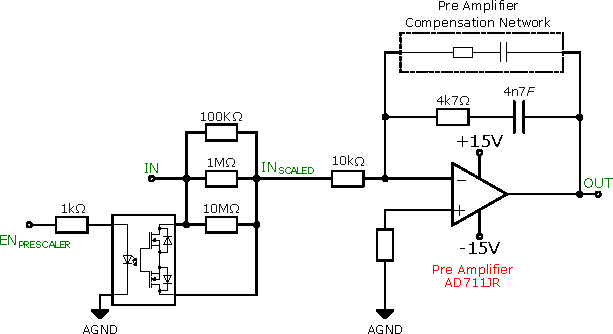
\includegraphics[width=0.85\textwidth]
    {figures/tests/preamp-test-circuit}
    \caption[Pre-Amplifier Isolation Test Circuit]{
        The equivalent circuit for testing the pre-amplifier in isolation.
    }
    \label{fig:test-preamp-isolation-circuit}
\end{figure}



The bandwidth measurements were carried out with an input voltage swing of
\SI{\pm10}{\volt}, once without prescaler\footnote{There is a relay-controlled divider network right before the input
stage that can divide the input signal by 10.} disabled and once with prescaler
set to $10:1$.

\subsection*{Measurement Results:}
With 8 resistors and 8 capacitors, a large combination of values is possible,
allowing us to fine-tune the bandwidth as required, therefore the results
presented here are for only a combination of one resistance value and 8
capacitance value.
The result is presented in \autoref{tab:combined_capacitor_bandwidth}.

\begin{table}[h!]
    \centering
    \resizebox{\linewidth}{!}{%
    \begin{tabular}{lcc}
        \toprule

        \small\textbf{Capacitor} & \small\textbf{B/W 3dB (Prescaler Disabled)} & \small\textbf{B/W 3dB (Prescaler 10:1)} \\
        \midrule
%        \SI{0}{\pico\farad}      & \SI{4200}{\kilo\hertz}                      & --                                      \\
        \SI{100}{\pico\farad}    & \SI{300}{\kilo\hertz}                       & \SI{225}{\kilo\hertz}                   \\
        \SI{220}{\pico\farad}    & \SI{120}{\kilo\hertz}                       & \SI{100}{\kilo\hertz}                   \\
        \SI{470}{\pico\farad}    & \SI{60}{\kilo\hertz}                        & \SI{50}{\kilo\hertz}                    \\
        \SI{1}{\nano\farad}      & \SI{30}{\kilo\hertz}                        & \SI{23}{\kilo\hertz}                    \\
        \SI{2.2}{\nano\farad}    & \SI{12}{\kilo\hertz}                        & \SI{9}{\kilo\hertz}                     \\
        \SI{4.7}{\nano\farad}    & \SI{6}{\kilo\hertz}                         & \SI{5}{\kilo\hertz}                     \\
        \SI{10}{\nano\farad}     & \SI{2.5}{\kilo\hertz}                       & \SI{2.4}{\kilo\hertz}                   \\
        \SI{22}{\nano\farad}     & \SI{1.2}{\kilo\hertz}                       & \SI{1.2}{\kilo\hertz}                   \\
        \bottomrule
    \end{tabular}
    }
    \caption[PreAmplifier Compensation Network Measurement]{
        Comparison of effect of changing capacitor values inthe compensation network of the pre amplifier.
    }
    \label{tab:combined_capacitor_bandwidth}
\end{table}

The difference in frequency between the results can be attributed to
signal amplitude and the capacitance of the analog relay used in the switching
of the prescaler divider network path.
It was observed that disabling the compensation will cause an
output resonance at \SI{5}{\mega\hertz} and the current draw of the amplifier
is \SI{13}{\milli\ampere} on average.

%! Author = Saeid Yazdani
%! Date = 9/6/2024


\section{Combined Pre and Power Amplifiers Measurements}
\label{sec:combined-preamp-paamp-meas}

The power amplifier (PA95) was analyzed for \emph{Current Consumption},
\emph{Settling Time} and \emph{Stability}.

\subsection{PA95 Current Consumption}

The PA95 draws asymmetrical currents from the supplies where the current draw
from the positive rail is on average \SI{10}{\percent} higher than the
current drawn from the negative rail.
On average, both currents are between \SI{1.8}{\milli\ampere} to
\SI{2.8}{\milli\ampere}, about  \SI{200}{\micro\ampere} higher than the
specified value in the datasheet (\SI{1.6}{\milli\ampere} to
\SI{2.2}{\milli\ampere}) \autocite{apex:pa95}.

Although the difference in the current draw is small, asymmetrical current
draw can cause ripple or
noise on the floating power supplies and may
manifest as nonlinear behavior or as a DC offset on the output signal.
This offset can be measured during calibration and digitally compensated by
adjusting the set-point signal inside the FPGA.

\subsection{Stability Analysis}

Using the \ac{MCU} for controlling \emph{Dynamic Gain Array} of the power
amplifier, as presented in \autoref{fig:power-amplifier}, stability
of the combined output of the pre amplifier and power amplifier was evaluated
at different gain settings.

With $G<10$, oscillating waveforms were observed at the PA95 output for all
compensation values of the preamplifier as shown in
\autoref{fig:pa-lowgain-meas}.

\begin{figure}[htbp]
    \centering
    \begin{minipage}{0.48\textwidth}
        \centering
        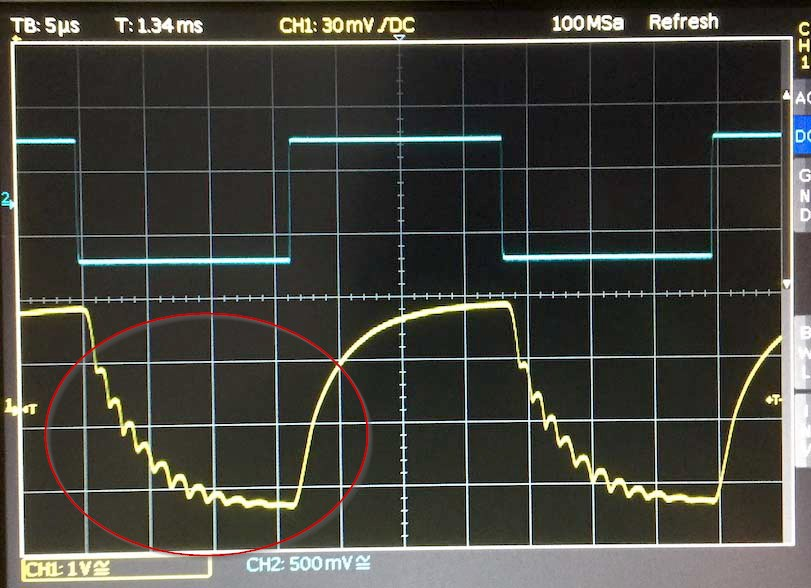
\includegraphics[width=\textwidth]{figures/tests/amptest/gain-lt10-precmp-low}
        \subcaption{Low Pre Amplifier B/W}
    \end{minipage}
    \hfill
    \begin{minipage}{0.47\textwidth}
        \centering
        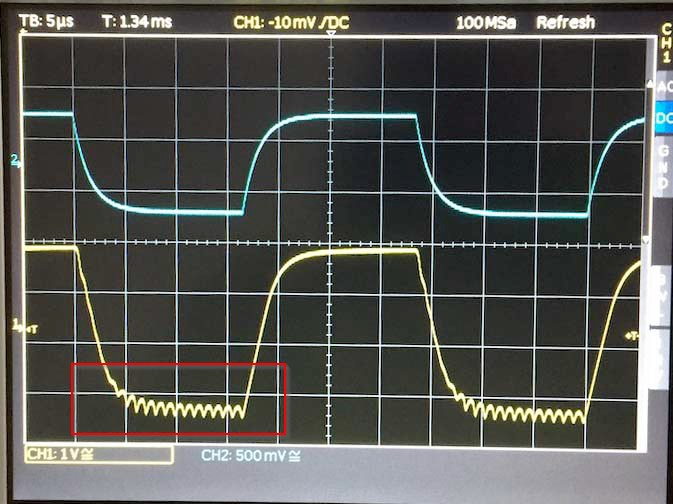
\includegraphics[width=\textwidth]{figures/tests/amptest/gain-lt10-precmp-high}
        \subcaption{High Pre Amplifier B/W}
    \end{minipage}
    \caption[Stability Measurement for $G < 10$ with Moderate B/W]{
        PA95 Stability Measurement for $G < 10$.
        \textbf{Blue Signal:} Pre Amplifier output.
        \textbf{Yellow Signal:} Power Amplifier output.
        \SI{5}{\micro\second} Timebase.
    }
    \label{fig:pa-lowgain-meas}
\end{figure}

Even with pre amplifier set to the maximum bandwidth, the oscillation still
appears on the falling edge as shown in \autoref{fig:pa-lowgain-pre-maxbw-meas}.

\begin{figure}[ht!]
    \centering
    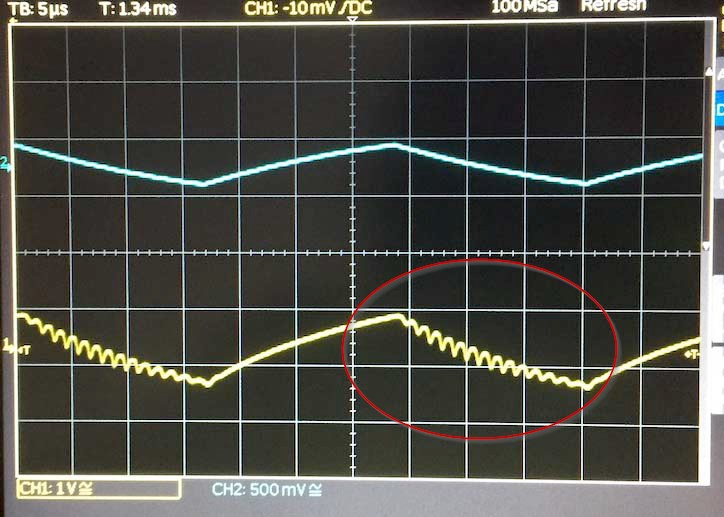
\includegraphics[width=0.52\textwidth]
    {figures/tests/amptest/gain-lt10-precmp-max}
    \caption[Stability Measurement for $G < 10$ with Max B/W]{
        Increasing the pre amplifier's bandwith to the maximum value does not
        remove the oscillation at the power amplifier's output.
        \SI{5}{\micro\second} Timebase.
    }
    \label{fig:pa-lowgain-pre-maxbw-meas}
\end{figure}

After thorough analysis, a few factors that can be attributed to this behavior
were identified:

\noindent\textbf{Lack of DC path:}
There was no DC path  in the local feedback of the pre amplifier as
depicted in \autoref{fig:test-preamp-isolation-circuit}.
A \acs{DC} path was added for stable operation as shown in
\autoref{fig:test-preamp-isolation-circuit-with-dc-path}.

\begin{figure}[h!]
    \centering
    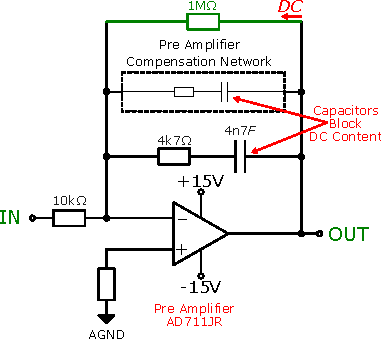
\includegraphics[width=0.6\textwidth]
    {figures/tests/preamp-test-circuit-with-dc-path}
    \caption[Pre-Amplifier With Added DC Path]{
        The capacitors in the series RC networks on the local feedback and
        compensation feedback block low-frequency DC content. Adding a
        resistor to the feedback path will allow DC content to flow.
    }
    \label{fig:test-preamp-isolation-circuit-with-dc-path}
\end{figure}

\noindent\textbf{Capacitance of relays in the feedback path:}
As stated before in \autoref{subsec:current-emasurement}, the compensation
network components and pre-scaler divider network are switched using analog
relays (\emph{OptoMOS} or \emph{PhotoMOS}) and the dynamic gain array uses
standard \acs{MOSFET}s which contribute to the total capacitance of the
control circuit.
The contribution of these stray capacitances
(up to \SI{50}{\pico\farad} per relay) must be taken into account in the
control loop processing.

\autoref {fig:gain-2dot4-with-stuff} shows the measurement repeated after
insertion of a resistor in the feedback path.
The oscillation at the falling edge is improved.

\begin{figure}[ht!]
    \centering
    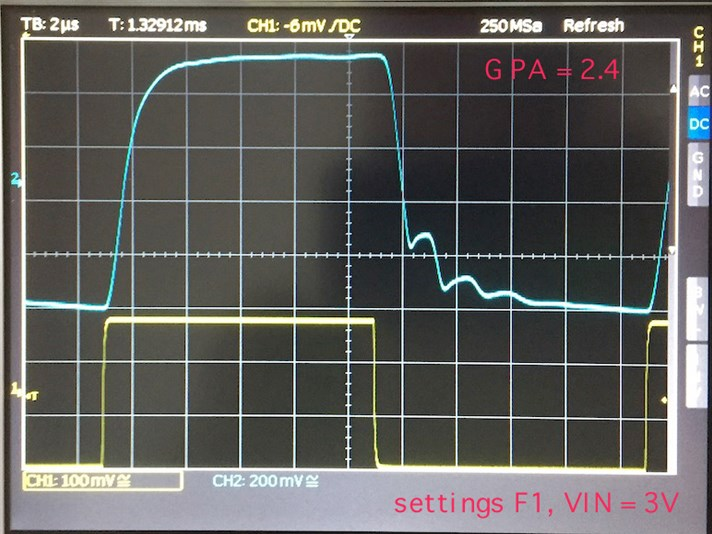
\includegraphics[width=0.52\textwidth]
    {figures/tests/amptest/gain-2dot4-with-stuff}
    \caption[Damped Oscillation]{
        The addition of a resistor for the DC path in the feedback has lowered the
        frequency content of the instability in the falling edge.
        \textbf{Blue Signal:} Power Amplifier output.
        \textbf{Yellow Signal:} Pre Amplifier output.
        \SI{5}{\micro\second} Timebase.
    }
    \label{fig:gain-2dot4-with-stuff}
\end{figure}
\subsection{Modification of PA95 Compensation Capacitor}
\label{subsec:modification-pa95-dedicated-comp}

High-gain or high-frequency operational amplifiers typically require
dedicated compensation capacitors to ensure stability and prevent unwanted
oscillations by design.
These capacitors are used for frequency compensation, which helps control the
amplifier's bandwidth and phase response.
This capacitor slows down the amplifier’s response to fast changes,
ensuring stable operation, especially in designs with feedback loops.

According to the power amplifier's datasheet \enquote{The PA95 is stable at
gains of 10 or more with
a compensation capacitor ($CC$) of 4.7pF mounted closely to pins 4 and 6 to prevent
spurious oscillation.
A compensation capacitor less than 4.7pF is not recommended}
\autocite{apex:pa95}.

The equivalent circuit presented in \autoref{fig:power-amplifier} shows this
capacitor connected to the $C_{COMP.}$ pins of the amplifier and actual value
is \SI{22}{\nano\farad}.
The placement on the \acs{PCB} layout is very close to the amplifier's pins
as depicted in \autoref{fig:pa95-cc-placement}.

\begin{figure}[t!]
    \centering
    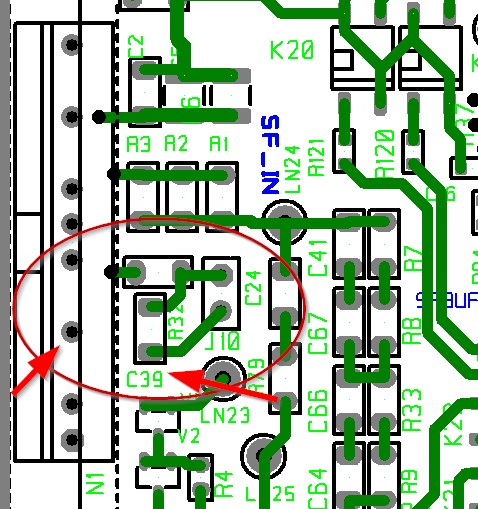
\includegraphics[width=0.6\textwidth]
    {figures/tests/amptest/pa95_cc_layout}
    \caption[PA95 $CC$ Placement]{
        The placement of the dedicated compensation capacitor for the power
        amplifier is optimal.
        \emph{N1} is the PA95 and \emph{C39} is the capacitor.
        A Series resistor \emph{R32} of \SI{10}{\ohm} is in series with the
        capacitor to dampen high-frequency oscillations.
        A Jumpr \emph{J10} is in parallel with \emph{C39}.
        \emph{J10} and \emph{R32} allow dropping in parallel and series
        capacitors to fine tune the compensation capacitor's final value.
    }
    \label{fig:pa95-cc-placement}
\end{figure}

A series of tests were carried out with different capacitor values, gain and
input voltages to verify the effect of the dedicated compensation capacitor on
power amplifier's output behavior.
This measurement results are presented in
\autoref{fig:pamp-cc-vs-gain} and verify that
a higher compensation capacitance for the power amplifier helps with reduction
of oscillation on the falling edge drastically.

\begin{figure}[htbp]
    \centering
    \captionsetup{font=footnotesize}
    \begin{minipage}{0.47\textwidth}
        \centering
        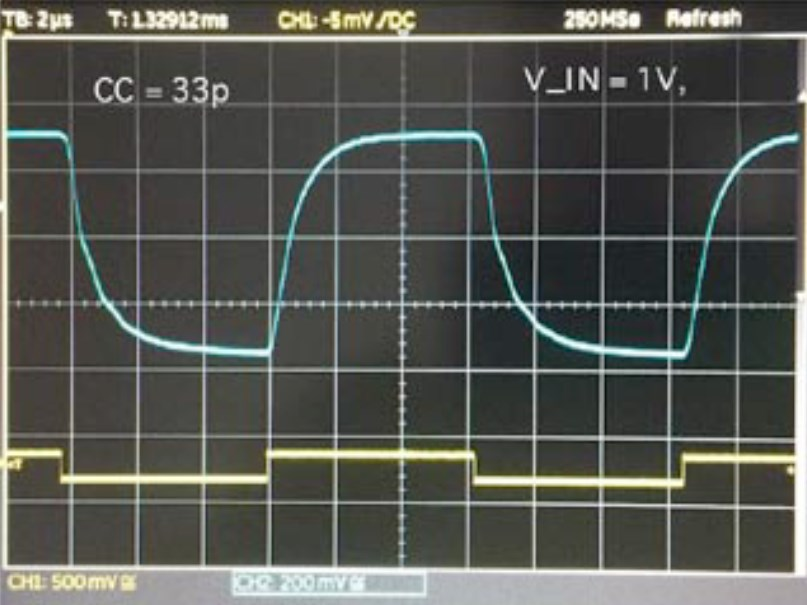
\includegraphics[width=\linewidth,height=0.18\textheight,keepaspectratio]{figures/tests/amptest/cc33-g2dot4-vin1}
        \subcaption{$G=2.4$, $C_C=33pF$ and $V_{IN}=1V$}\label{fig:cc33-g2dot4-vin1}
    \end{minipage}
    \hfill
    \begin{minipage}{0.47\textwidth}
        \centering
        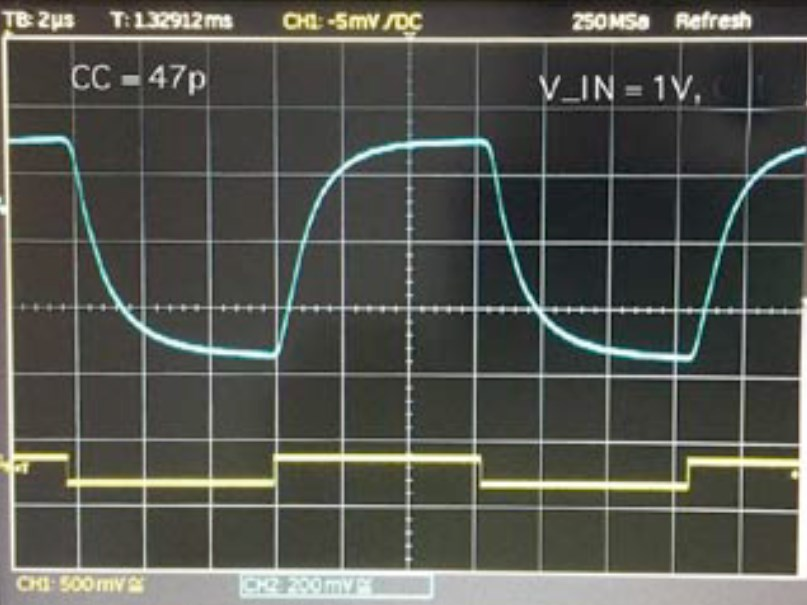
\includegraphics[width=\linewidth,height=0.18\textheight,keepaspectratio]{figures/tests/amptest/cc47-g2dot4-vin1}
        \subcaption{$G=2.4$, $C_C=47pF$ and $V_{IN}=1V$}\label{fig:cc47-g2dot4-vin1}
    \end{minipage}

    \vspace{0.12cm}

    \begin{minipage}{0.47\textwidth}
        \centering
        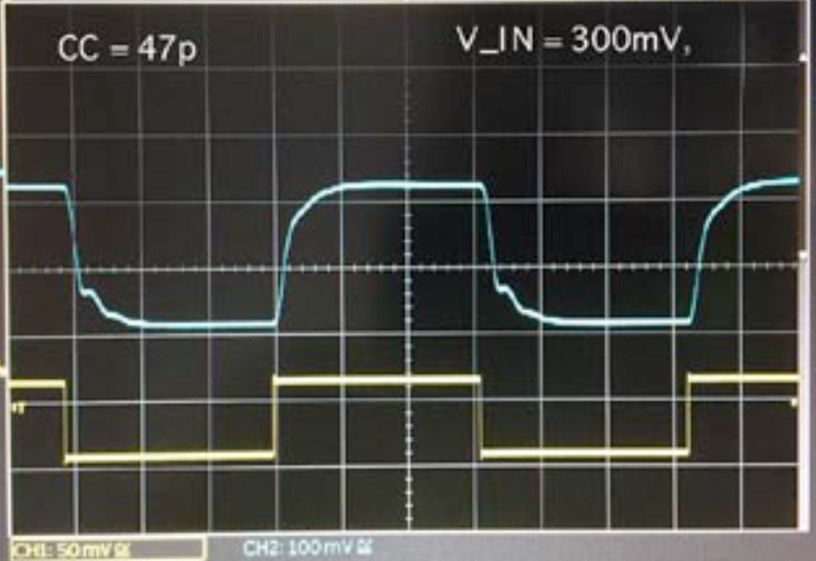
\includegraphics[width=\linewidth,height=0.18\textheight,keepaspectratio]{figures/tests/amptest/cc47-g2dot4-vin0dot300}
        \subcaption{$G=2.4$, $C_C=47pF$ and $V_{IN}=300mV$}\label{fig:cc47-g2dot4-vin0dot300}
    \end{minipage}
    \hfill
    \begin{minipage}{0.47\textwidth}
        \centering
        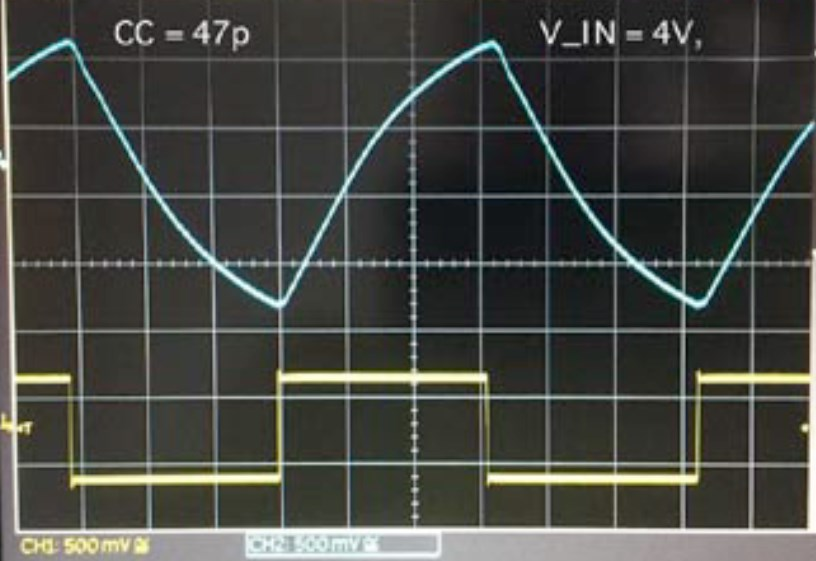
\includegraphics[width=\linewidth,height=0.18\textheight,keepaspectratio]{figures/tests/amptest/cc47-g2dot4-vin4}
        \subcaption{$G=2.4$, $C_C=47pF$ and $V_{IN}=4V$}\label{fig:cc47-g2dot4-vin4}
    \end{minipage}

    \vspace{0.12cm}

    \begin{minipage}{0.47\textwidth}
        \centering
        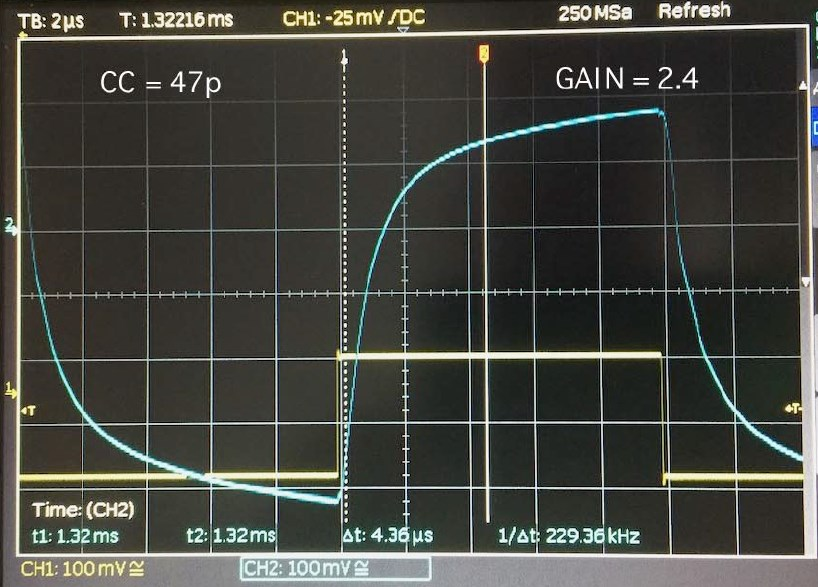
\includegraphics[width=\linewidth,height=0.18\textheight,keepaspectratio]{figures/tests/amptest/cc47-g2dot4-or10}
        \subcaption{$G=2.4$, $C_C=47pF$ and $V_{IN}=6V$}\label{fig:cc47-g2dot4-or10}
    \end{minipage}
    \hfill
    \begin{minipage}{0.47\textwidth}
        \centering
        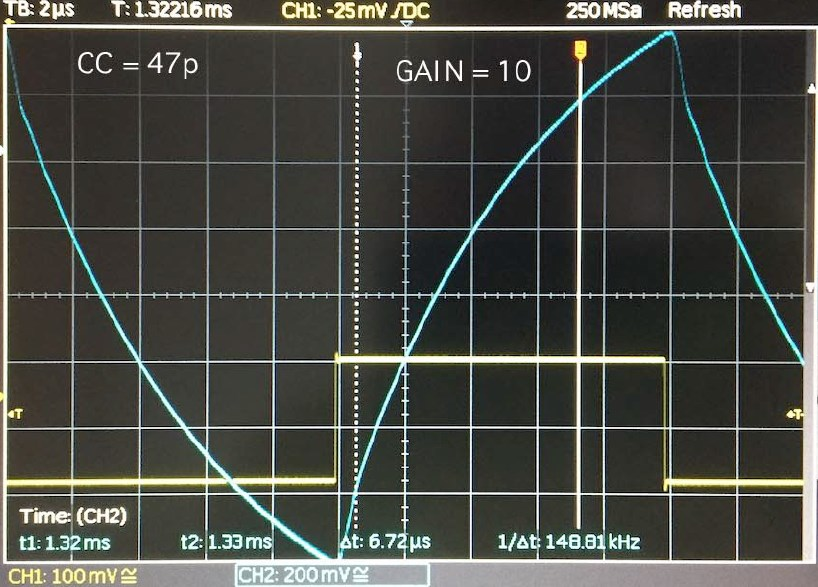
\includegraphics[width=\linewidth,height=0.18\textheight,keepaspectratio]{figures/tests/amptest/cc47-g10}
        \subcaption{$G=10$, $C_C=47pF$ and $V_{IN}=6V$}\label{fig:cc47-g10}
    \end{minipage}

    \caption[PA95 Dedicated Compensation Capacitor Effect]{
        Effects of PA95 dedicated $C_{COMP.}$ on the output based on
        various gain settings and input voltages.
        \textbf{Blue Signal:} Power Amplifier output.
        \textbf{Yellow Signal:} Pre Amplifier output.
        \SI{2}{\micro\second} Timebase.
    }
    \label{fig:pamp-cc-vs-gain}
\end{figure}

\subsection{Conclusion}
\label{subsec:amplifiers-conclusion}

The following points summarize the findings obtained by the measurements:
\begin{itemize}[topsep=8pt,itemsep=4pt,partopsep=4pt, parsep=4pt]
    \item The pre amplifier needs a DC feedback path.
    \item The divider stage requires a buffering amplifier for compensation.
    \item The power amplifier's higher gains result in a limited slew rate.

    \item The power amplifier's dedicated compensation capacitor must be
    increased.
    \item Swing range of the pre amplifier needs adjustment.
\end{itemize}

\clearpage

%! Author = Saeid Yazdani
%! Date = 9/7/2024


\section{Source-Follower Measurements}
\label{source-follower-measurements}

As stated before, the source follower multiplies the current
capabilities of the power amplifier according to the transconductance of the
used \acs{MOSFET}s on the high and low sides.
A series of measurements were carried out on the source-follower to
find design issues and perform optimization.

The bias currents of the LEDs are measured to be around \SI{1}{\milli\ampere} and
a voltage drop of \SI{1.6}{\volt} at high differential resistance.

The high-side \acs{MOSFET} (IXFH14N80P) shows an input capacitance of
\SI{3.9}{\nano\farad} and for the low-side \acs{MOSFET} (IXFH16P60P)
\SI{5.2}{\nano\farad}.

The small difference of the gate capacitances of the high-side and
low-side \acs{MOSFET}s leads to an imbalance in
turn-on and turn-off timings, since the gate capacitance determines how
quickly the \acs{MOSFET}s turn on or off.

The gate capacitance mismatch affects the load handling conditions as the slower
\acs{MOSFET} leads to less efficient energy transfer or higher stress on
the other \acs{MOSFET}.

Therefore, the gate drivers for both \acs{MOSFET}s must be adjusted in a way
that the difference in switching times is minimized.
This can be achieved by altering the current and/or voltage used for driving
each \acs{MOSFET}.


\begin{figure}[h!]
    \centering
    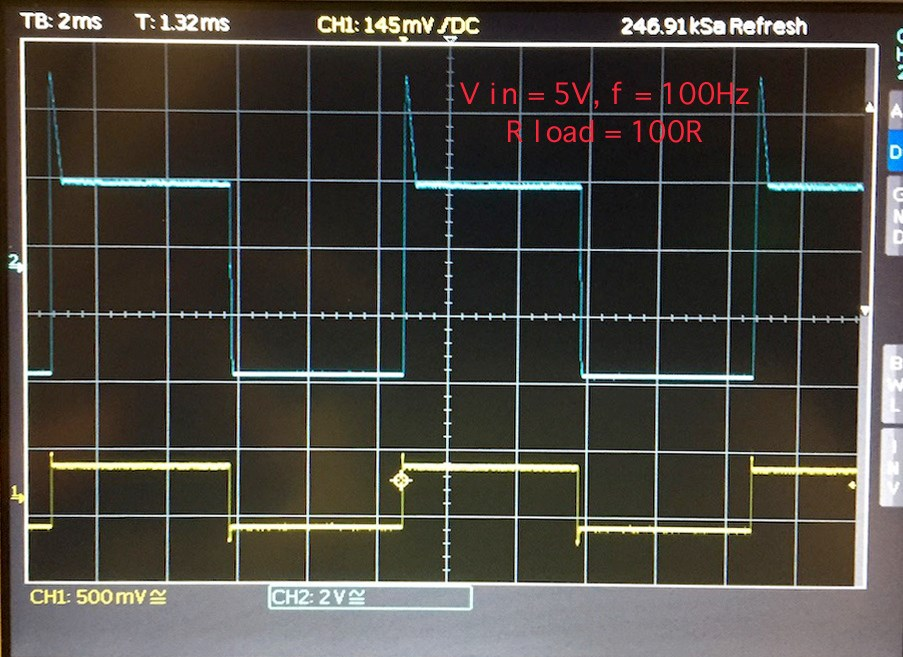
\includegraphics[scale=0.32]
    {figures/tests/amptest/sf_static}
    \caption[Power Stage Static Behavior]{
        Static behaviour of the power stage for a \SI{100}{\hertz}
        signal.
        $V_{IN}$ = \SI{5}{\volt} and $R_{LOAD}$ = \SI{100}{\ohm}
        \textbf{Blue Signal:} Source-Follower output.
        \textbf{Yellow Signal:} Pre Amplifier output.
        \SI{2}{\milli\second} Timebase.
    }
    \label{fig:power-stage-static-behacior}
\end{figure}


\begin{figure}[ht]
    \centering
    \begin{minipage}{0.48\textwidth}
        \centering
        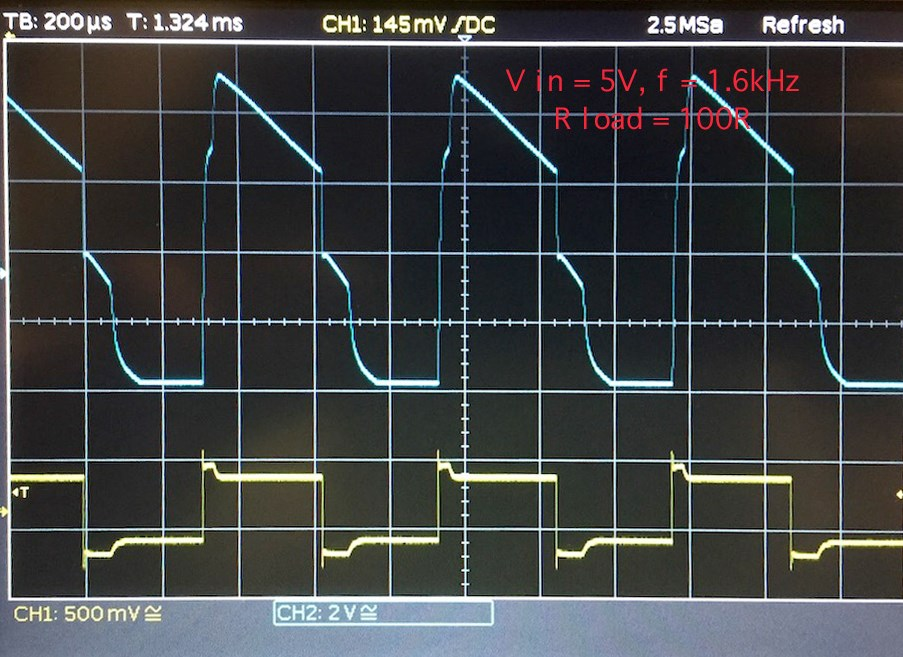
\includegraphics[width=\textwidth]{figures/tests/amptest/sf_dynamic-1dot6khz}
        \subcaption{$V_{IN}$ = \SI{5}{\volt}, $Freq.$ = \SI{1.6}{\kilo\hertz} and $R_{LOAD}$ = \SI{100}{\ohm}}
    \end{minipage}
    \hfill
    \begin{minipage}{0.48\textwidth}
        \centering
        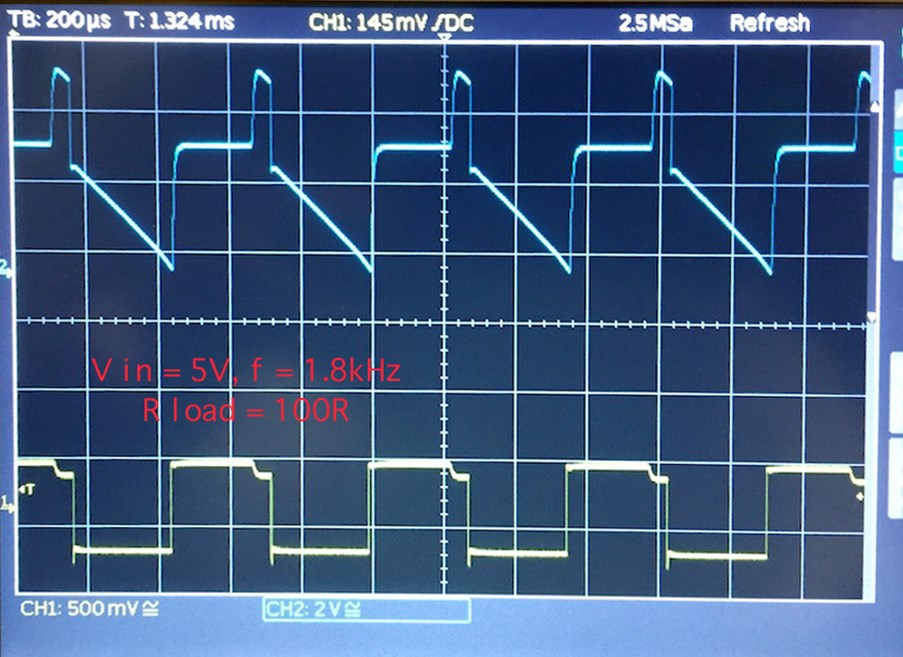
\includegraphics[width=\textwidth]{figures/tests/amptest/sf_dynamic-1dot8khz}
        \subcaption{$V_{IN}$ = \SI{5}{\volt}, $Freq.$ = \SI{1.8}{\kilo\hertz} and $R_{LOAD}$ = \SI{100}{\ohm}}
    \end{minipage}
    \caption[Power Stage Dynamic Behavior]{
        Dynamic behavior of the power stage. Stop frequency is \SI{1.8}{\kilo\hertz}.
        \textbf{Blue Signal:} Source-Follower output.
        \textbf{Yellow Signal:} Pre Amplifier output.
        \SI{200}{\micro\second} Timebase.
    }
    \label{fig:power-stage-dynamic-behacior}
\end{figure}

%! Author = Saeid Yazdani
%! Date = 9/8/2024


\section{Functional Tests}
\label{sec:functional-tests}

The system as a whole was evaluated with functional tests to verify that it
operates according to design specifications and performs the intended functions:

\begin{itemize}[topsep=8pt,itemsep=4pt,partopsep=4pt, parsep=4pt]
    \item \textbf{Firmware/Software Integration:}
    ensures that the software controlling the hardware is working properly,
    and safety guards are engaging correctly.

    \item \textbf{Signal and Data Flow Validation:}
    Verify that inputs result in correct outputs, communication protocol is
    working properly, and relays and sensors are responding as expected.

    \item \textbf{Real-World Scenarios:}
    Simulating real-world operational conditions, including testing at
    different voltages, temperatures, loads and stability in extended
    operation times.

\end{itemize}

Multiple instruments
are used for the calibration of voltage and current values and for
cross-measuring system's input and output for functional validation.
\autoref{fig:hvs-development-rack} shows the development rack and the supporting
equipment.

\begin{figure}[p]
    \centering
    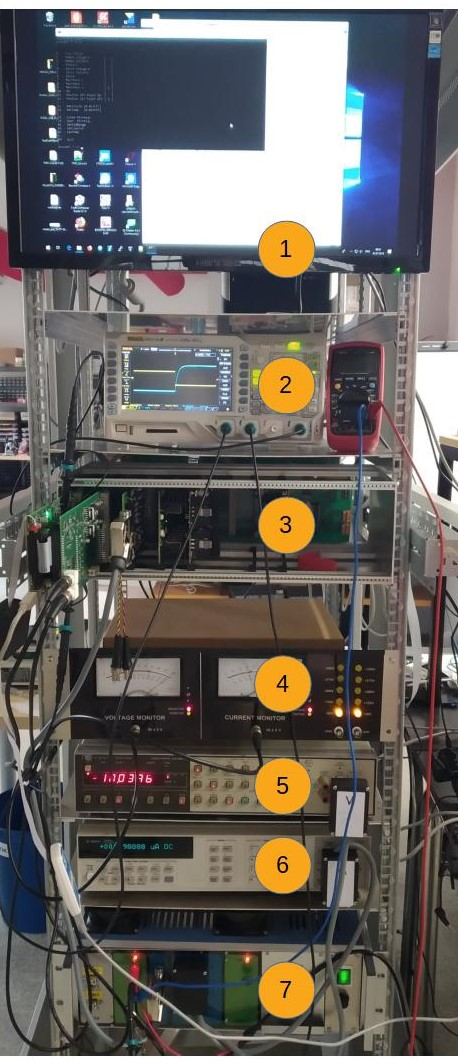
\includegraphics[width=\linewidth,height=0.85\textheight,keepaspectratio]
    {figures/prototype/production/image12}
    \caption[System Test Rack]{
        The \acs{HVS} system test and development tower.
        \textbf{(1)} A PC for executing the operator software.
        \textbf{(2)} Oscilloscope for signal debugging.
        \textbf{(3)} The \ac{HVS}.
        \textbf{(4)} Analog meters connected to the monitor board.
        \textbf{(5)} Multimeter for voltage measurements.
        \textbf{(6)} Multimeter for current measurements.
        \textbf{(7)} Custom-made array of switchable resistive loads.
    }
    \label{fig:hvs-development-rack}
\end{figure}

\subsection{Full-Swing Tests}
\label{subsec:full-swing-tests}

% 600V Swing
\autoref{fig:640v_swing_no_compensation} shows the \acs{HVS} response to
a full-range \SI{\pm320}{\volt}
swing from the negative to the positive quadrant without any compensation.
The transition from \SI{-300}{\volt} to \SI{+300}{\volt} has a settling time of
\SI{250}{\micro\second} and slight overshoot of \SI{25}{\volt} which is a
remarkable and on par with premium high-voltage power supplies in the market.

\begin{figure}[htbp]
    \centering
    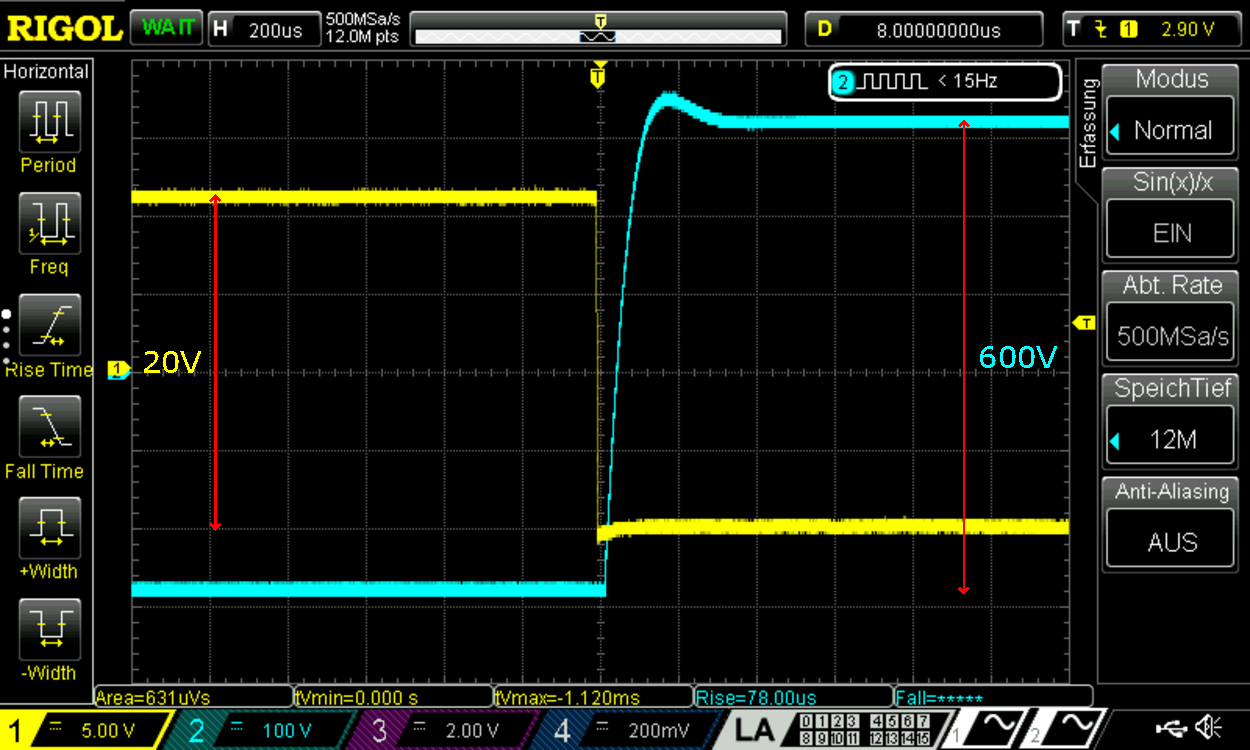
\includegraphics[width=\textwidth]
    {figures/tests/640v_swing_no_compensation}
    \caption[\SI{\pm300}{\volt} Swing Test With No Compensation]{
        Without dynamic compensation, the \acs{HVS} achieved a
        full range swing of \SI{600}{\volt}, settling time of
        \SI{250}{\micro\second} and slight overshoot of \SI{20}{\volt}.
        The control signal is inverted.
        \textbf{Blue Signal:} \acs{HVS} Output (\SI{100}{\volt} per division).
        \textbf{Yellow Signal:} Pre Amplifier output (\SI{5}{\volt} per division).
        \SI{200}{\micro\second} Timebase.
    }
    \label{fig:640v_swing_no_compensation}
\end{figure}

\begin{figure}[htbp]
    \centering
    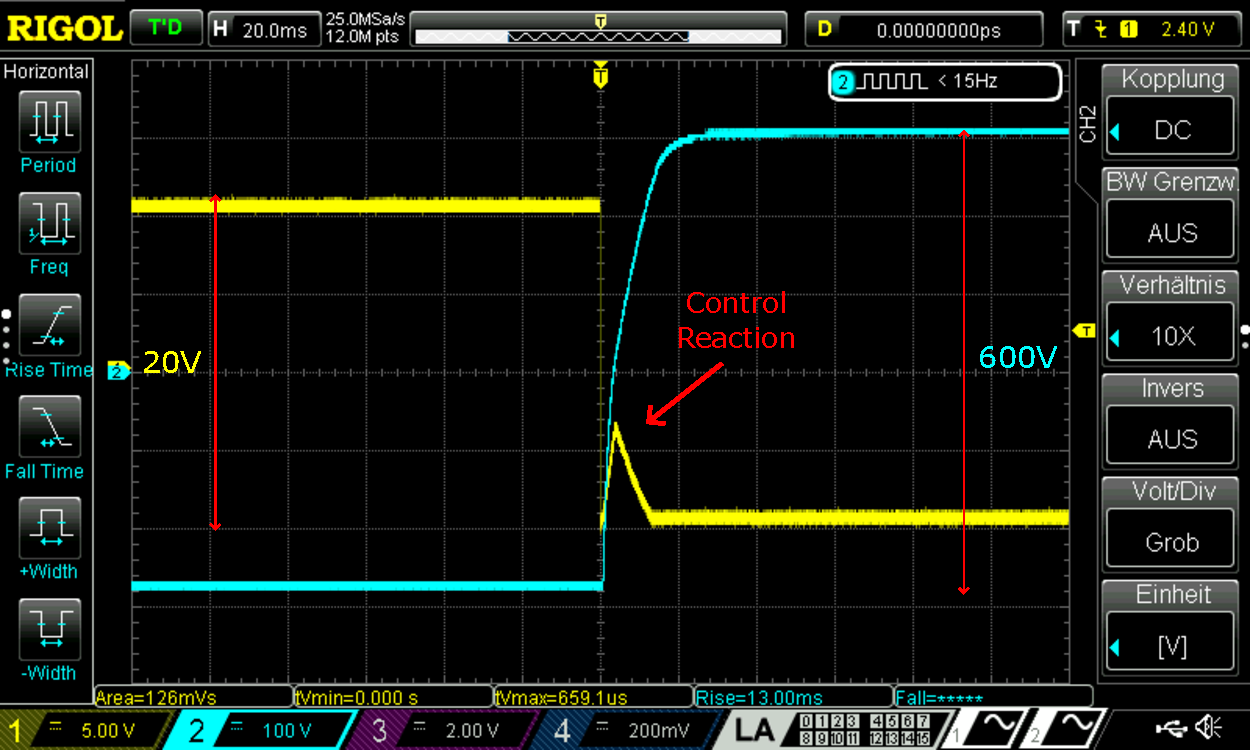
\includegraphics[width=\textwidth]
    {figures/tests/640v_swing_with_compensation}
    \caption[\SI{\pm320}{\volt} Swing Test With Dynamic Compensation]{
        By engaging the dynamic compensation, the \acs{HVS} achieved a
        swing of \SI{600}{\volt} and settling time of
        \SI{22}{\milli\second} without any \emph{overshoot}.
        The bounce visible on the pre amplifier signal issued by the FPGA
        compensates and suppresses the overshoot.
        \textbf{Blue Signal:} \acs{HVS} Output (\SI{100}{\volt} per division).
        \textbf{Yellow Signal:} Pre Amplifier output (\SI{5}{\volt} per division).
        \SI{20}{\milli\second} Timebase.
    }
    \label{fig:640v_swing_with_compensation}
\end{figure}

% With the application of dynamic compensation
% to adapt the power stage to the \ac{DUT}'s specific needs.
\autoref{fig:640v_swing_with_compensation} shows the same test setup but with
the dynamic compensation enabled.
This time, the overshoot is suppressed by the control loop where near the peak
of the voltage swing control signal performs the adjustments to prevent the
overshoot.
The achieved settling time in this mode is \SI{20}{\milli\second} that is
increased by a factor of 80.

% 20V swing
The result of a half-range swing test for the lower range of \SI{\pm10}{\volt}
with dynamic compensation enabled is shown in \autoref{fig:0Vto8V_swing_with_compensation}.
In this test, the voltage swings from \SI{-4}{\volt} to \SI{+4}{\volt}
with a settling time of \SI{4}{\milli\second} with no overshoot.

\begin{figure}[h!]
    \centering
    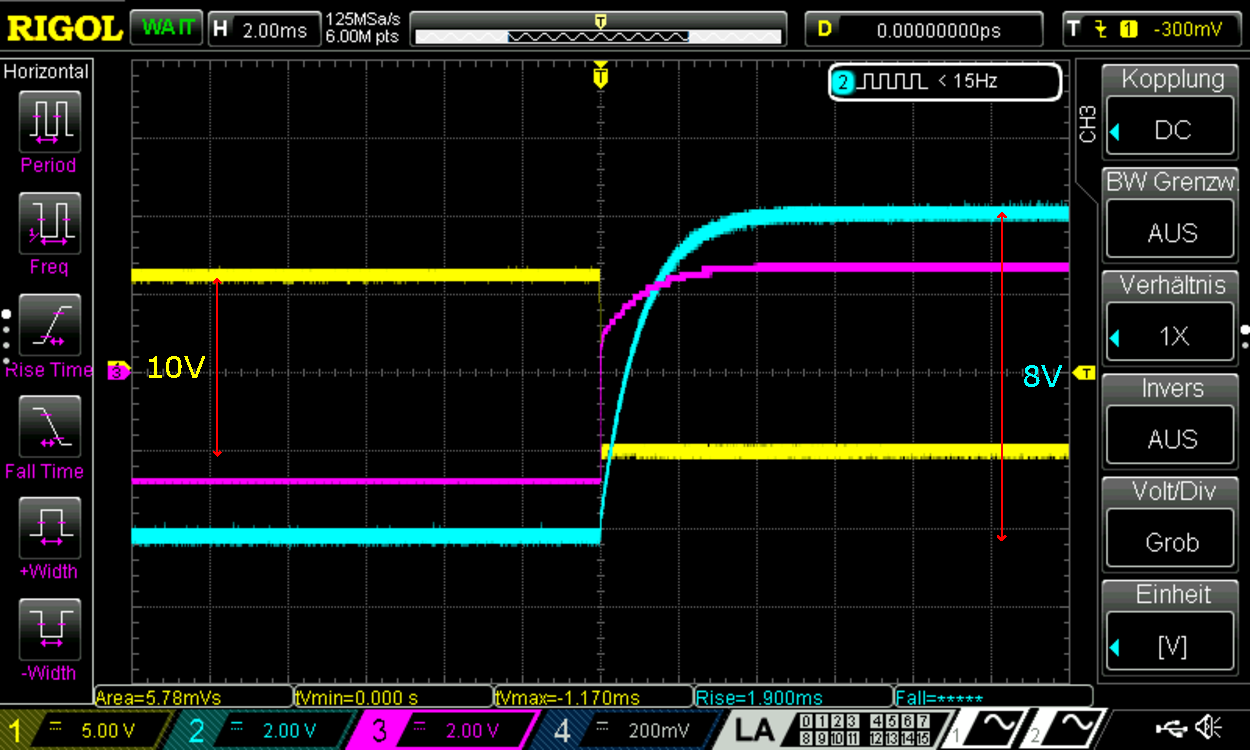
\includegraphics[width=\textwidth]
    {figures/tests/10v_positive_swing_with_compensation}
    \caption[\SI{\pm10}{\volt} Swing Test With Dynamic Compensation]{
        With dynamic compensation enabled, the \acs{HVS} manages to swing
        from \SI{-4}{\volt} to \SI{+4}{\volt} in \SI{4}{\milli\second}
        without any overshoot for a resistive load of \SI{75}{\ohm}.
        \textbf{Blue Signal:} \acs{HVS} Output (\SI{2}{\volt} per division).
        \textbf{Pink Signal:} Current Signal (\SI{50}{\milli\ampere} per division).
        \textbf{Yellow Signal:} Pre Amplifier output (\SI{5}{\volt} per division).
        \SI{2}{\milli\second} Timebase.
    }
    \label{fig:0Vto8V_swing_with_compensation}
\end{figure}

\subsection{Enduring Stability Test}
\label{subsec:longtime-stability-test}

To test the long-term stability of the \acs{HVS}, it was used as a constant
current source in a platform for testing the reliability of
\acs{PCB} traces and interconnects under harsh environments developed at
TU Chemnitz \autocite{9547972}.

In this test method, a power supply is required to force a constant current
with a minimum amount of deviation for a long period into a series
chain of traces with multiple vias on a large \acs{PCB}.
The test \acs{PCB} then is inserted in a thermal chamber and undergoes
temperature cycling in \SI{20}{\degreeCelsius} to \SI{140}{\degreeCelsius}
range.
A fixed current is necessary to measure changes in the resistance over a
typical period of one month or until a trace fails-open due to via barrel
crack or delamination. The test elements and their description are presented in
\autoref{fig:hvs-as-current-source-in-pcb-tester}.

\clearpage
The \acs{HVS} managed to effectively yield on par results with another
industry standard lab power supply over a period of two weeks until the
tests stopped.
Sample sof these measurement results are presented in
\autoref{fig:via-chain-results}.

\begin{figure}[ht]
    \centering

    % Top figure
    \begin{minipage}{\textwidth}
        \centering
        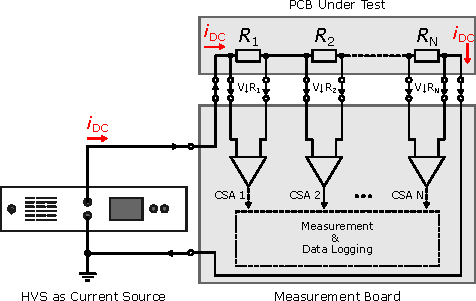
\includegraphics[width=0.75\textwidth]{figures/tests/via-chain-equivallent-circuit}
        \subcaption{Equivallend circuit of the \acs{PCB} reliability test method.
        }
        \label{fig:top}
    \end{minipage}

    % Space between figures
    \vspace{1em}

    % Two figures side by side
    \begin{minipage}{0.49\textwidth}
        \centering
        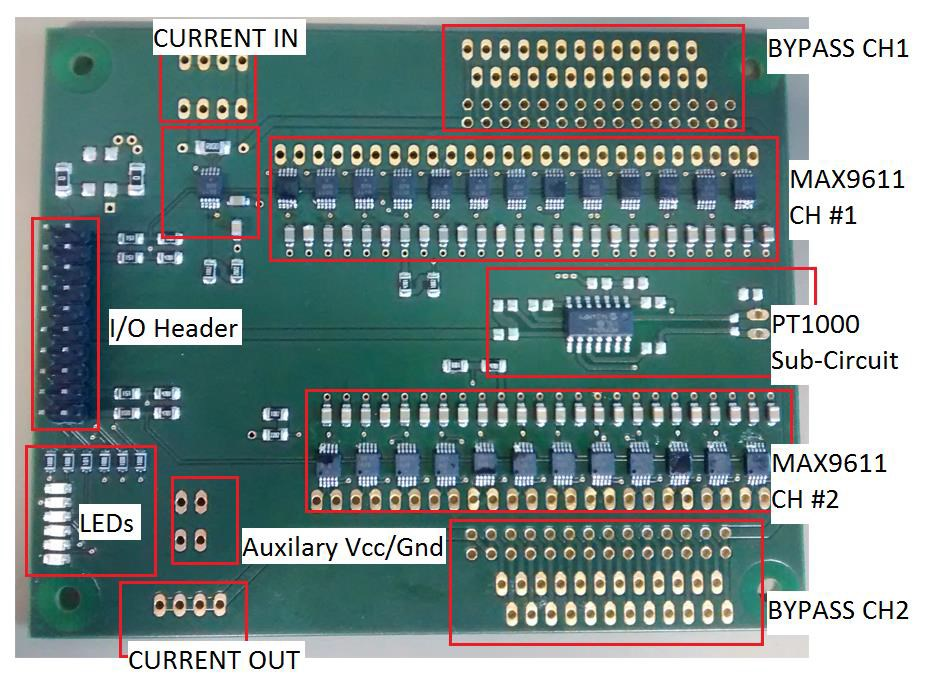
\includegraphics[width=\textwidth]{figures/tests/via-chain-measurement-board}
        \subcaption{Control board for wiring and data-logging.}
        \label{fig:bottomleft}
    \end{minipage}
    \hfill
    \begin{minipage}{0.49\textwidth}
        \centering
        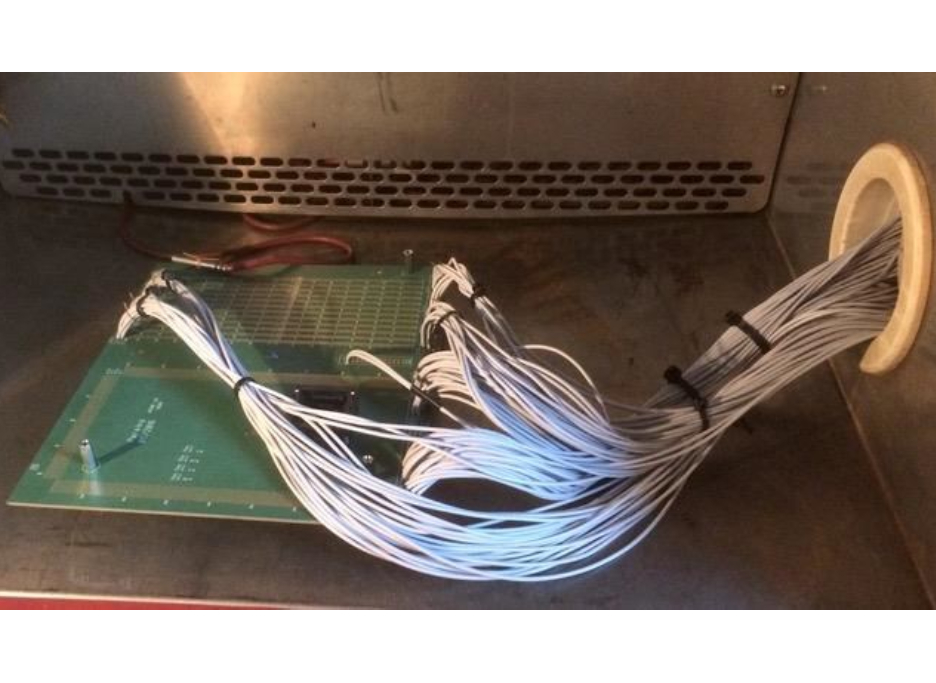
\includegraphics[width=\textwidth]{figures/tests/via-chain-in-oven}
        \subcaption{The \acs{PCB} test coupon inserted into a thermal chamber.
        }
        \label{fig:bottomright}
    \end{minipage}

    \caption[\acs{HVS} as Current Source in \acs{PCB} Reliability Test Platform]{
        A Constant current goes through each \acs{PCB} trace/interconnect on the
        test \acs{PCB}. These interconnects acts as a shunt resistor for their
        dedicated \ac{CSA}.
        Since the amount of current is known, the resulting voltage drop will
        yield the resistance of the interconnect under test.
        The changes in resistance at different temperatures will be recorded
        over time and deviations from the initial state will be studied.
    }
    \label{fig:hvs-as-current-source-in-pcb-tester}
\end{figure}

\begin{figure}[ht!]
    \centering
    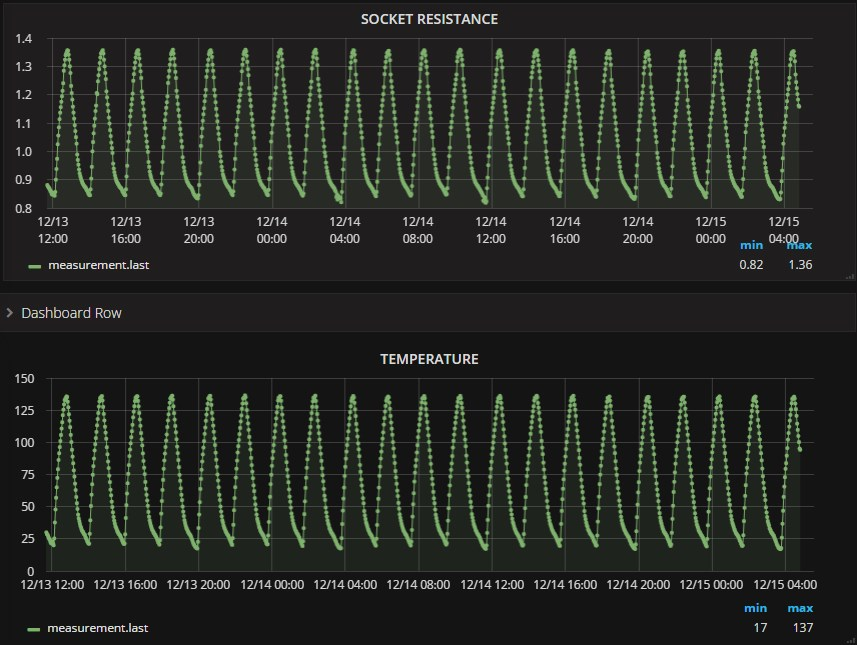
\includegraphics[width=0.8\textwidth]
    {figures/tests/via-chain-results}
    \caption[\acs{HVS} Long-Term Test Sample Result]{
        Measurement results of an interconnect on the test \acs{PCB} Under Test.
        Over two days the resistance of the interconnect has increased and
        decreased linearly against the temperature.
        The \acs{HVS} was used as a current source to apply a known stable current at
        fixed intervals for measuring the resistance according to the voltage drop
        over the interconnect.
    }
    \label{fig:via-chain-results}
\end{figure}

%! Author = Saeid Yazdani
%! Date = 9/9/2024


\section{Conclusion and Future Work}
\label{sec:conclusion-and-future-work}

\subsection{Conclusion}

The scope of this work was to demonstrate the applicability of a hybrid
digital-analog approach for power supply design with a dynamic compensation
scheme for the testing of semiconductors in \acs{ATE} systems.

Advancements in FPGA logic size and speed have enabled the implementation of
real-time adaptive control schemes.
These advancements provide the means to address the challenges presented by
modern semiconductor devices, particularly in ensuring high-quality power
delivery during testing.

The primary focus of this work was the optimization of signal waveforms at
the pins of \acs{DUT}s, where anomalies such as ringing, overshoot, and
undershoot in the supply rails can significantly degrade test quality and yield.
These anomalies could damage the \acs{DUT} in worst-case scenarios.
This issue is critical because, although modern devices may survive short
overvoltage pulses such as ringing, their long-term reliability can be
compromised due to the potential latent failures induced during the test phase
and only show up in the field.

As a result, the quality of power rail waveforms is of utmost importance.
Fast rise and fall times without ringing are essential to avoid any
potential degradation in device behavior.
This work demonstrated that safe and predictable waveforms can be achieved
through adaptive feedback control, where parameter sets are switched dynamically
— similar to the adaptive positioning systems used in fast robotics.

One of the key challenges discussed in this research was the limitation
of current-generation \acs{ATE} \acs{DPS}, which are often used in
ganged-mode to provide the necessary currents for demanding \acs{DUT}s.
This mode comes with its own set of challenges.
A single power supply that can provide the necessary current at all common
voltage levels would be the more flexible solution as proposed in this work.

A prototype system was developed to validate the advantages of this hybrid
approach.
Challenges and shortcomings encountered in the proposed
three-stage driver circuit were studied and solutions were provided.

Measurements demonstrated that modern \acs{FPGA}, \acs{ADC}, and \acs{DAC}
components allow for rapid responses, which are critical for maintaining
the stability and precision of the power delivery system.

The primary limitation observed was the amplitude-discrete nature of digital
signals.
To overcome this, cascaded converters with coarse and vernier stages were
developed, achieving the necessary amplitude resolution for precise control.

In conclusion, this work has successfully demonstrated the feasibility and
advantages of a hybrid digital-analog approach in \acs{ATE} systems, providing
a pathway for future improvements in semiconductor testing and ensuring more
robust, reliable device behavior during and after the test phase.

\subsection{Future Work}


\noindent\textbf{Upgrading the Digital Block:}

Between the time of starting this research work and the time of writing this
text, the \acs{FPGA} technology has seen technological leaps in several key
areas driven by the need for higher performance and improved design flexibility.
The \acs{HVS} can benefit from new generation of \acs{FPGA} chips
in the following areas:

\begin{itemize}[topsep=8pt,itemsep=4pt,partopsep=4pt, parsep=4pt]
    \item \textbf{Integration of Artificial Intelligence:}
    FPGAs have significantly evolved to support \ac{AI} and \ac{ML} workloads.
    Many FPGA families now include dedicated AI engines, such as \ac{TPU} or
    other neural network accelerators, built into the fabric.
    These advancements make FPGAs highly competitive for edge AI and machine
    learning applications that can benefit the \acs{HVS}'s adaptive
    compensation scheme.

    \item \textbf{SoC Integration:}
    FPGAs have become highly integrated heterogeneous platforms and feature
    hardware based embedded processors (e.g., ARM Cortex cores).
    The \acs{HVS} can significantly benefit from the speed up of
    communication between the operator software and the FPGA,
    lower design complexity and smaller footprint on the \ac{PCB}
    by replacing the discrete \acs{MCU} by an integrated one.

    \item \textbf{High-Speed \acs{I/O}:}
    Modern \acs{FPGA}s support much higher data rates, often exceeding
    \SI{100}{\giga\bit\per\second} for transceivers, and they offer built-in
    support for the latest connectivity standards such as 6th generation
    \acs{PCIe} and fast \acs{DDR}5.
    A high \ac{I/O} speed of the \acs{FPGA} in \acs{HVS} can aalow for faster
    data transactions.
    Including high-speed external memory can extend the acquisition memory
    used for both control loop and datapoint storage.

\end{itemize}

\pagebreak
\noindent\textbf{Upgrading the Analog Block:}

Just like \acs{FPGA}s, there are new and faster power amplifiers,
\acs{ADC}s and \acs{DAC}s available on the market.
For the current booster stage, upgrading from silicon-based \acs{MOSFET}s to
wide bandgap \acs{MOSFET}s (\emph{Silicon Carbide} or \emph{Gallium Nitride})
can be beneficial in achieving faster response rates.
\emph{Silicon Carbide} offers lower on-resistance
and reduced switching losses, which increases efficiency at higher frequencies.
Faster switching speeds and high thermal conductivity of such \acs{MOSFET}s
are essential factors to consider.
These new technologies should be evaluated in future iterations of the
\acs{HVS}.

\noindent\textbf{Synchronization of Multiple \acs{HVS} Units:}

Exact synchronization between \acs{DPS} units is mandatory
for modern devices with multiple voltage rail requirements (e.g., \SI{5}{\volt}
for analog, \SI{3.3}{\volt} for I/O, and \SI{1.3}{\volt}
for core supplies) as otherwise there is a high risk of latch-up.
To mitigate this, a fixed startup sequence for all individual supply rails is
necessary.
As the proposed system voltages are monitored digitally, this setup phase can
be easily programmed between multiple units of the proposed system to ensure
proper sequencing and avoid related failures.

\noindent\textbf{Integration in Recognized ATE Systems:}

The \acs{HVS} prototype was developed and tested as a stand-alone
\acs{DPS}/\acs{SMU}.
Integration of this system in industry-standard \ac{ATE} systems requires
direct collaboration with \acs{ATE} manufacturers.
The current iteration of the \acs{HVS} offers a simple but effective communication
protocol, and library files for easy integration are well prepared.
Another option to expose the \acs{HVS} to other hardware is the integration of
the \acs{HVS}'s \acs{API} as an extension to the already available
\emph{SpecScribe} \autocite{markert, schott}, a specification tool for analog
hardware developed at TU Chemnitz.

\noindent\textbf{Moving to a Single Board Design:}

The current iteration of the \acs{HVS} hardware uses the backplane-based
prototyping approach. The driver stage, analog frontend and control boards
are the most critical sections of the hardware where any signal distortion can
affect the overall behavior of the system.
The signals travel through multiple connectors and the backplane to
reach their destination.
Because of this, the communication rates between system components are not
at their maximum as the priority in the prototype was
the proof of functionality.
By combining critical sections of the hardware in one board problems can
be avoided and maximum transfer rates can be achieved.



